% Options for packages loaded elsewhere
\PassOptionsToPackage{unicode}{hyperref}
\PassOptionsToPackage{hyphens}{url}
\PassOptionsToPackage{dvipsnames,svgnames,x11names}{xcolor}
%
\documentclass[
  letterpaper,
  DIV=11,
  numbers=noendperiod]{scrartcl}

\usepackage{amsmath,amssymb}
\usepackage{iftex}
\ifPDFTeX
  \usepackage[T1]{fontenc}
  \usepackage[utf8]{inputenc}
  \usepackage{textcomp} % provide euro and other symbols
\else % if luatex or xetex
  \usepackage{unicode-math}
  \defaultfontfeatures{Scale=MatchLowercase}
  \defaultfontfeatures[\rmfamily]{Ligatures=TeX,Scale=1}
\fi
\usepackage{lmodern}
\ifPDFTeX\else  
    % xetex/luatex font selection
\fi
% Use upquote if available, for straight quotes in verbatim environments
\IfFileExists{upquote.sty}{\usepackage{upquote}}{}
\IfFileExists{microtype.sty}{% use microtype if available
  \usepackage[]{microtype}
  \UseMicrotypeSet[protrusion]{basicmath} % disable protrusion for tt fonts
}{}
\makeatletter
\@ifundefined{KOMAClassName}{% if non-KOMA class
  \IfFileExists{parskip.sty}{%
    \usepackage{parskip}
  }{% else
    \setlength{\parindent}{0pt}
    \setlength{\parskip}{6pt plus 2pt minus 1pt}}
}{% if KOMA class
  \KOMAoptions{parskip=half}}
\makeatother
\usepackage{xcolor}
\setlength{\emergencystretch}{3em} % prevent overfull lines
\setcounter{secnumdepth}{5}
% Make \paragraph and \subparagraph free-standing
\makeatletter
\ifx\paragraph\undefined\else
  \let\oldparagraph\paragraph
  \renewcommand{\paragraph}{
    \@ifstar
      \xxxParagraphStar
      \xxxParagraphNoStar
  }
  \newcommand{\xxxParagraphStar}[1]{\oldparagraph*{#1}\mbox{}}
  \newcommand{\xxxParagraphNoStar}[1]{\oldparagraph{#1}\mbox{}}
\fi
\ifx\subparagraph\undefined\else
  \let\oldsubparagraph\subparagraph
  \renewcommand{\subparagraph}{
    \@ifstar
      \xxxSubParagraphStar
      \xxxSubParagraphNoStar
  }
  \newcommand{\xxxSubParagraphStar}[1]{\oldsubparagraph*{#1}\mbox{}}
  \newcommand{\xxxSubParagraphNoStar}[1]{\oldsubparagraph{#1}\mbox{}}
\fi
\makeatother

\usepackage{color}
\usepackage{fancyvrb}
\newcommand{\VerbBar}{|}
\newcommand{\VERB}{\Verb[commandchars=\\\{\}]}
\DefineVerbatimEnvironment{Highlighting}{Verbatim}{commandchars=\\\{\}}
% Add ',fontsize=\small' for more characters per line
\usepackage{framed}
\definecolor{shadecolor}{RGB}{241,243,245}
\newenvironment{Shaded}{\begin{snugshade}}{\end{snugshade}}
\newcommand{\AlertTok}[1]{\textcolor[rgb]{0.68,0.00,0.00}{#1}}
\newcommand{\AnnotationTok}[1]{\textcolor[rgb]{0.37,0.37,0.37}{#1}}
\newcommand{\AttributeTok}[1]{\textcolor[rgb]{0.40,0.45,0.13}{#1}}
\newcommand{\BaseNTok}[1]{\textcolor[rgb]{0.68,0.00,0.00}{#1}}
\newcommand{\BuiltInTok}[1]{\textcolor[rgb]{0.00,0.23,0.31}{#1}}
\newcommand{\CharTok}[1]{\textcolor[rgb]{0.13,0.47,0.30}{#1}}
\newcommand{\CommentTok}[1]{\textcolor[rgb]{0.37,0.37,0.37}{#1}}
\newcommand{\CommentVarTok}[1]{\textcolor[rgb]{0.37,0.37,0.37}{\textit{#1}}}
\newcommand{\ConstantTok}[1]{\textcolor[rgb]{0.56,0.35,0.01}{#1}}
\newcommand{\ControlFlowTok}[1]{\textcolor[rgb]{0.00,0.23,0.31}{\textbf{#1}}}
\newcommand{\DataTypeTok}[1]{\textcolor[rgb]{0.68,0.00,0.00}{#1}}
\newcommand{\DecValTok}[1]{\textcolor[rgb]{0.68,0.00,0.00}{#1}}
\newcommand{\DocumentationTok}[1]{\textcolor[rgb]{0.37,0.37,0.37}{\textit{#1}}}
\newcommand{\ErrorTok}[1]{\textcolor[rgb]{0.68,0.00,0.00}{#1}}
\newcommand{\ExtensionTok}[1]{\textcolor[rgb]{0.00,0.23,0.31}{#1}}
\newcommand{\FloatTok}[1]{\textcolor[rgb]{0.68,0.00,0.00}{#1}}
\newcommand{\FunctionTok}[1]{\textcolor[rgb]{0.28,0.35,0.67}{#1}}
\newcommand{\ImportTok}[1]{\textcolor[rgb]{0.00,0.46,0.62}{#1}}
\newcommand{\InformationTok}[1]{\textcolor[rgb]{0.37,0.37,0.37}{#1}}
\newcommand{\KeywordTok}[1]{\textcolor[rgb]{0.00,0.23,0.31}{\textbf{#1}}}
\newcommand{\NormalTok}[1]{\textcolor[rgb]{0.00,0.23,0.31}{#1}}
\newcommand{\OperatorTok}[1]{\textcolor[rgb]{0.37,0.37,0.37}{#1}}
\newcommand{\OtherTok}[1]{\textcolor[rgb]{0.00,0.23,0.31}{#1}}
\newcommand{\PreprocessorTok}[1]{\textcolor[rgb]{0.68,0.00,0.00}{#1}}
\newcommand{\RegionMarkerTok}[1]{\textcolor[rgb]{0.00,0.23,0.31}{#1}}
\newcommand{\SpecialCharTok}[1]{\textcolor[rgb]{0.37,0.37,0.37}{#1}}
\newcommand{\SpecialStringTok}[1]{\textcolor[rgb]{0.13,0.47,0.30}{#1}}
\newcommand{\StringTok}[1]{\textcolor[rgb]{0.13,0.47,0.30}{#1}}
\newcommand{\VariableTok}[1]{\textcolor[rgb]{0.07,0.07,0.07}{#1}}
\newcommand{\VerbatimStringTok}[1]{\textcolor[rgb]{0.13,0.47,0.30}{#1}}
\newcommand{\WarningTok}[1]{\textcolor[rgb]{0.37,0.37,0.37}{\textit{#1}}}

\providecommand{\tightlist}{%
  \setlength{\itemsep}{0pt}\setlength{\parskip}{0pt}}\usepackage{longtable,booktabs,array}
\usepackage{calc} % for calculating minipage widths
% Correct order of tables after \paragraph or \subparagraph
\usepackage{etoolbox}
\makeatletter
\patchcmd\longtable{\par}{\if@noskipsec\mbox{}\fi\par}{}{}
\makeatother
% Allow footnotes in longtable head/foot
\IfFileExists{footnotehyper.sty}{\usepackage{footnotehyper}}{\usepackage{footnote}}
\makesavenoteenv{longtable}
\usepackage{graphicx}
\makeatletter
\def\maxwidth{\ifdim\Gin@nat@width>\linewidth\linewidth\else\Gin@nat@width\fi}
\def\maxheight{\ifdim\Gin@nat@height>\textheight\textheight\else\Gin@nat@height\fi}
\makeatother
% Scale images if necessary, so that they will not overflow the page
% margins by default, and it is still possible to overwrite the defaults
% using explicit options in \includegraphics[width, height, ...]{}
\setkeys{Gin}{width=\maxwidth,height=\maxheight,keepaspectratio}
% Set default figure placement to htbp
\makeatletter
\def\fps@figure{htbp}
\makeatother
% definitions for citeproc citations
\NewDocumentCommand\citeproctext{}{}
\NewDocumentCommand\citeproc{mm}{%
  \begingroup\def\citeproctext{#2}\cite{#1}\endgroup}
\makeatletter
 % allow citations to break across lines
 \let\@cite@ofmt\@firstofone
 % avoid brackets around text for \cite:
 \def\@biblabel#1{}
 \def\@cite#1#2{{#1\if@tempswa , #2\fi}}
\makeatother
\newlength{\cslhangindent}
\setlength{\cslhangindent}{1.5em}
\newlength{\csllabelwidth}
\setlength{\csllabelwidth}{3em}
\newenvironment{CSLReferences}[2] % #1 hanging-indent, #2 entry-spacing
 {\begin{list}{}{%
  \setlength{\itemindent}{0pt}
  \setlength{\leftmargin}{0pt}
  \setlength{\parsep}{0pt}
  % turn on hanging indent if param 1 is 1
  \ifodd #1
   \setlength{\leftmargin}{\cslhangindent}
   \setlength{\itemindent}{-1\cslhangindent}
  \fi
  % set entry spacing
  \setlength{\itemsep}{#2\baselineskip}}}
 {\end{list}}
\usepackage{calc}
\newcommand{\CSLBlock}[1]{\hfill\break\parbox[t]{\linewidth}{\strut\ignorespaces#1\strut}}
\newcommand{\CSLLeftMargin}[1]{\parbox[t]{\csllabelwidth}{\strut#1\strut}}
\newcommand{\CSLRightInline}[1]{\parbox[t]{\linewidth - \csllabelwidth}{\strut#1\strut}}
\newcommand{\CSLIndent}[1]{\hspace{\cslhangindent}#1}

\usepackage{booktabs}
\usepackage{longtable}
\usepackage{array}
\usepackage{multirow}
\usepackage{wrapfig}
\usepackage{float}
\usepackage{colortbl}
\usepackage{pdflscape}
\usepackage{tabu}
\usepackage{threeparttable}
\usepackage{threeparttablex}
\usepackage[normalem]{ulem}
\usepackage{makecell}
\usepackage{xcolor}
\usepackage{caption}
\usepackage{anyfontsize}
\usepackage{tabularray}
\usepackage[normalem]{ulem}
\usepackage{graphicx}
\UseTblrLibrary{booktabs}
\UseTblrLibrary{rotating}
\UseTblrLibrary{siunitx}
\NewTableCommand{\tinytableDefineColor}[3]{\definecolor{#1}{#2}{#3}}
\newcommand{\tinytableTabularrayUnderline}[1]{\underline{#1}}
\newcommand{\tinytableTabularrayStrikeout}[1]{\sout{#1}}
\KOMAoption{captions}{tableheading}
\makeatletter
\@ifpackageloaded{caption}{}{\usepackage{caption}}
\AtBeginDocument{%
\ifdefined\contentsname
  \renewcommand*\contentsname{Table of contents}
\else
  \newcommand\contentsname{Table of contents}
\fi
\ifdefined\listfigurename
  \renewcommand*\listfigurename{List of Figures}
\else
  \newcommand\listfigurename{List of Figures}
\fi
\ifdefined\listtablename
  \renewcommand*\listtablename{List of Tables}
\else
  \newcommand\listtablename{List of Tables}
\fi
\ifdefined\figurename
  \renewcommand*\figurename{Figure}
\else
  \newcommand\figurename{Figure}
\fi
\ifdefined\tablename
  \renewcommand*\tablename{Table}
\else
  \newcommand\tablename{Table}
\fi
}
\@ifpackageloaded{float}{}{\usepackage{float}}
\floatstyle{ruled}
\@ifundefined{c@chapter}{\newfloat{codelisting}{h}{lop}}{\newfloat{codelisting}{h}{lop}[chapter]}
\floatname{codelisting}{Listing}
\newcommand*\listoflistings{\listof{codelisting}{List of Listings}}
\makeatother
\makeatletter
\makeatother
\makeatletter
\@ifpackageloaded{caption}{}{\usepackage{caption}}
\@ifpackageloaded{subcaption}{}{\usepackage{subcaption}}
\makeatother

\ifLuaTeX
  \usepackage{selnolig}  % disable illegal ligatures
\fi
\usepackage{bookmark}

\IfFileExists{xurl.sty}{\usepackage{xurl}}{} % add URL line breaks if available
\urlstyle{same} % disable monospaced font for URLs
\hypersetup{
  pdftitle={My title},
  pdfauthor={First author; Another author},
  colorlinks=true,
  linkcolor={blue},
  filecolor={Maroon},
  citecolor={Blue},
  urlcolor={Blue},
  pdfcreator={LaTeX via pandoc}}


\title{My title\thanks{Code and data are available at:
\url{https://github.com/RohanAlexander/starter_folder}.}}
\usepackage{etoolbox}
\makeatletter
\providecommand{\subtitle}[1]{% add subtitle to \maketitle
  \apptocmd{\@title}{\par {\large #1 \par}}{}{}
}
\makeatother
\subtitle{My subtitle if needed}
\author{First author \and Another author}
\date{December 3, 2024}

\begin{document}
\maketitle
\begin{abstract}
First sentence. Second sentence. Third sentence. Fourth sentence.
\end{abstract}


\section{Introduction}\label{introduction}

Child care subsidies play a critical role in making high-quality early
childhood education and care accessible to families and communities. In
Toronto, licensed child care centres serve as essential providers,
offering regulated and professional environments that support child
development. Subsidies for licensed child care centres help close the
affordability gap by offsetting the high costs of quality care, making
it accessible to more families (Cleveland and Krashinsky 2009). These
subsidies not only ease the financial burden on families but also ensure
that children have access to nurturing environments that foster
cognitive, social, and emotional growth during their formative years
(Vines 2020). Understanding the factors that determine which licensed
centres receive subsidies is crucial for policymakers and stakeholders
to promote equitable resource allocation and maximize the benefits of
early childhood programs. Licensed child care centres in urban settings
like Toronto play a pivotal role in delivering high-quality, structured
child care. These centres adhere to stringent regulations, ensuring
compliance with standards for safety, staffing, and curriculum. Research
highlights that children attending licensed centres, particularly those
supported by subsidies, experience better developmental outcomes (Adams
et al., 2013). Subsidized centres provide professional environments with
trained educators, comprehensive programming, and age-appropriate
resources, offering children a strong foundation for lifelong learning
and success (Herbst, 2014). Subsidies are a cornerstone of this
ecosystem, enabling licensed centres to cover operational costs, retain
qualified staff, and maintain compliance with regulatory standards, all
of which enhance the quality of care provided (Ryan et al. 2011).
Despite their importance, disparities in the allocation of subsidies
remain a significant concern. Research indicates that centres in certain
neighborhoods or serving specific populations may receive fewer
subsidies, even when demand is high (Johnson, Ryan, and Brooks‐Gunn
2012). Additionally, characteristics such as enrollment capacity,
accreditation status, and program focus (e.g., infant care versus
pre-kindergarten) often influence a centre's eligibility and
prioritization for funding (\textbf{vines2020accessin?}). These
discrepancies highlight the need for a data-driven approach to
understanding and improving the distribution of subsidies among licensed
child care centres, ensuring that resources are allocated equitably to
maximize their impact. This study utilizes the Toronto Open Data:
Licensed Child Care Centres dataset to explore the factors that affect
subsidy allocation to licensed centres. By analyzing variables such as
ward, operating auspice (Commercial, Non Profit or Public), CWELCC, type
of building, and total space, this research aims to uncover the question
- ``What factors influence the allocation of subsidies to licensed child
care centres in Toronto?''. The findings will contribute to informing
policies that promote equity and efficiency in subsidy allocation,
ultimately supporting the goals of accessible and high-quality child
care in Toronto. Additionally, these insights can serve as a valuable
tool for child care centres to self-assess and enhance their eligibility
for subsidies.

Telegraphing paragraph: The remainder of this paper is structured as
follows. Section~\ref{sec-data}\ldots.

\section{Data}\label{sec-data}

\subsection{Data Overview}\label{data-overview}

The dataset used in this study was sourced from the
(\textbf{Childrens\_Services?}) made publicly available by the City of
Toronto. This original raw dataset provides detailed information about
licensed child care centres, including 20 variables capturing aspects of
their location, operating auspice (e.g., non-profit, public, or
commercial), space usage, building type, participation in government
programs such as the Canada-Wide Early Learning and Child Care (CWELCC)
system, and other operational details. These data offer valuable
insights into the factors influencing subsidy allocation, a key policy
tool for improving access to early childhood education and care. By
translating real-world phenomena into structured data entries, this
dataset enables a comprehensive exploration of equity and efficiency in
child care funding. Detailed data collection analysis is in appendix

\begin{Shaded}
\begin{Highlighting}[]
\NormalTok{data }\OtherTok{\textless{}{-}} \FunctionTok{read.csv}\NormalTok{(}\StringTok{"../data/02{-}analysis\_data/cleaned\_data.csv"}\NormalTok{)}
\end{Highlighting}
\end{Shaded}

\begin{table}

\caption{\label{tbl-overview}Sample of Cleaned Data}

\centering{

\caption*{
{\large Overview of Cleaned Data} \\ 
{\small Displaying the first 10 rows}
} 
\fontsize{12.0pt}{14.4pt}\selectfont
\begin{tabular*}{\linewidth}{@{\extracolsep{\fill}}rllrrr}
\toprule
ward & AUSPICE & bldg\_type & cwelcc\_flag & TOTSPACE & subsidy \\ 
\midrule\addlinespace[2.5pt]
3 & Non Profit Agency & Public Elementary School & 1 & 164 & 1 \\ 
8 & Non Profit Agency & Public Elementary School & 1 & 83 & 1 \\ 
25 & Non Profit Agency & Catholic Elementary School & 1 & 102 & 1 \\ 
10 & Non Profit Agency & Other & 1 & 65 & 1 \\ 
20 & Non Profit Agency & High Rise Apartment & 1 & 26 & 1 \\ 
24 & Non Profit Agency & Community College/University & 1 & 62 & 1 \\ 
6 & Non Profit Agency & Public High School & 1 & 49 & 1 \\ 
24 & Commercial Agency & High Rise Apartment & 1 & 46 & 1 \\ 
19 & Non Profit Agency & Public Elementary School & 1 & 51 & 1 \\ 
8 & Non Profit Agency & Public Elementary School & 1 & 153 & 1 \\ 
\bottomrule
\end{tabular*}

}

\end{table}%

\begin{figure}

\centering{

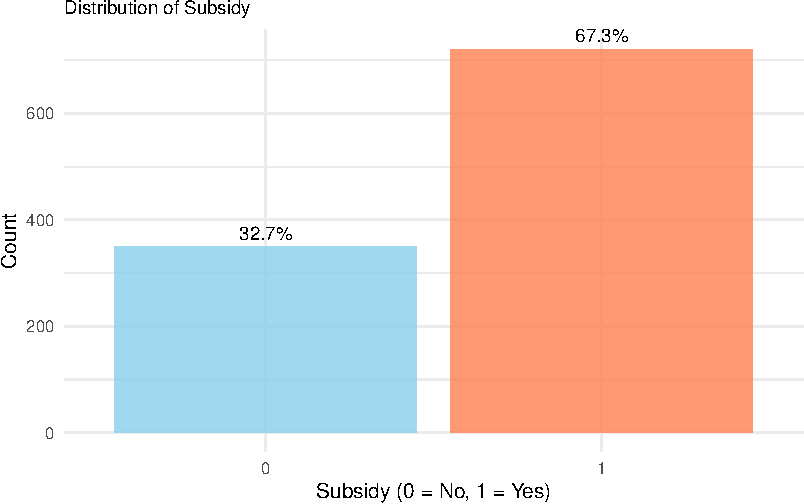
\includegraphics{paper_files/figure-pdf/fig-subsidy-1.pdf}

}

\caption{\label{fig-subsidy}Subsidy Allocation Distribution}

\end{figure}%

\subsection{Method}\label{method}

The dataset used for this study is the
\textbf{\texttt{Licensed\ Child\ Care\ Centres\ dataset}}, sourced from
the (Gelfand 2022) It provides detailed information about licensed child
care centres in Toronto, capturing aspects such as their governance,
capacity, infrastructure, and subsidy status. The original dataset
consisted of 1071 records for all licensed child care centres within the
city. For this analysis, the data underwent preprocessing to focus on
variables relevant to the study, such as subsidy status, building type,
CWELCC participation, total space, and operating auspice. These
variables were retained to examine how different factors influence
subsidy allocation. The dependent variable \textbf{\texttt{subsidy}},
originally recorded as ``Yes''/``No,'' was encoded as 1 for subsidized
and 0 for non-subsidized centres. Similarly, the
\textbf{\texttt{cwelcc\_flag}} variable was converted into a binary
format (1 =Y, 0 =N). Categorical variables such as
\textbf{\texttt{bldg\_type}} and \textbf{\texttt{AUSPICE}} were
consolidated to simplify analysis and address sparse categories.
Additionally, missing and irrelevant records were removed to ensure the
dataset was both accurate and meaningful for the research objectives.

The data for this study was systematically downloaded, cleaned,
analyzed, and visualized using \textbf{\texttt{R}} (R Core Team 2023), a
statistical programming language. The following are major packages used
for this study: \textbf{\texttt{opendatatoronto}}(Gelfand 2022): Used to
access and retrieve the Licensed Child Care Centres dataset directly
from the City of Toronto's open data portal. \textbf{\texttt{readr}}
(Wickham, Hester, and Bryan 2024): Simplified the import and parsing of
raw data into R. \textbf{\texttt{tidyverse}} (Wickham et al. 2019):
Streamlined data manipulation, cleaning, and visualization processes.
\textbf{\texttt{dplyr}} (Wickham et al. 2023): Provided tools for
filtering, transforming, and summarizing the dataset effectively.
\textbf{\texttt{ggplot2}} (Wickham 2016): Created powerful and flexible
visualizations tailored to the analysis needs. \textbf{\texttt{car}}
(Fox and Weisberg 2019): Used for diagnostic tools, including Variance
Inflation Factor (VIF) tests, to assess multicollinearity.
\textbf{\texttt{caret}} (Kuhn and Max 2008): Enabled the development,
validation, and evaluation of machine learning models, including
training-test splits and performance metrics. \textbf{\texttt{glmnet}}
(Friedman et al., 2010): Applied for fitting regularized regression
models and feature selection. \textbf{\texttt{stargazer}} (Hlavac 2022):
Generated formatted regression tables for outputs.
\textbf{\texttt{knitr}} (Xie 2021): Dynamically integrated code,
results, and plots into the final document for seamless reporting. \#\#
Measurement This analysis focuses on the following variables, with a
specific emphasis on subsidy as the dependent variable:
\texttt{subsidy}: The binary dependent variable indicating whether a
licensed child care centre receives a government subsidy. 1: The centre
is subsidized. 0: The centre is not subsidized. \texttt{ward}:
\texttt{A\ numeric\ variable\ representing\ the\ ward\ number\ for\ child\ care\ centres.}AUSPICE\texttt{:\ The\ operating\ auspice\ of\ the\ child\ care\ centre,\ describing\ its\ governance\ and\ operational\ model.\ Possible\ values\ include:\ Non-Profit:\ Centres\ operated\ by\ non-profit\ organizations,\ often\ reinvesting\ surplus\ revenues\ into\ quality\ improvements.\ Commercial:\ For-profit\ centres\ operated\ by\ private\ organizations.\ Public:\ Centres\ run\ by\ public\ agencies\ or\ school\ boards.}bldg\_type\texttt{:\ The\ type\ of\ building\ where\ the\ child\ care\ centre\ operates,\ reflecting\ its\ infrastructure.\ Examples\ include:\ bldg\_typeCommercial\ Building\ bldg\_typeCommunity\ College/University\ \ \ \ \ \ bldg\_typeCommunity\ Health\ Centre\ bldg\_typeCommunity\ Rec/Centre\ -\ Board\ Run\ bldg\_typeCommunity/Rec\ Centre\ -\ City\ bldg\_typeCommunity/Recreation\ Centre\ bldg\_typeHigh\ Rise\ Apartment\ bldg\_typeHospital/Health\ Centre\ bldg\_typeHouse\ bldg\_typeIndustrial\ Building\ bldg\_typeLow\ Rise\ Apartment\ bldg\_typeOffice\ Building\ bldg\_typeOther\ bldg\_typePlace\ of\ Worship\ bldg\_typePrivate\ Elementary\ School\ bldg\_typePublic\ (school\ closed)\ bldg\_typePublic\ Elementary\ Special\ bldg\_typePublic\ High\ School\ bldg\_typePublic\ Middle\ School\ bldg\_typePurpose\ Built\ bldg\_typeSynagogue}cwelcc\_flag\texttt{:\ A\ binary\ variable\ indicating\ participation\ in\ the\ Canada-Wide\ Early\ Learning\ and\ Child\ Care\ (CWELCC)\ program:\ 1:\ The\ centre\ participates\ in\ CWELCC,\ enabling\ reduced\ child\ care\ fees.\ 0:\ The\ centre\ does\ not\ participate\ in\ CWELCC.}TOTSPACE`:
A numerical variable representing the total licensed capacity (spaces
available) for all age groups at a child care centre. Detailed
information about these variables' information and data structure is
presented in Table~\ref{tbl-overview}.

The variables were carefully selected based on literature-supported
relevance to subsidy allocation and their representation of real-world
phenomena

Figure~\ref{fig-relationbldgtype} illustrates the distribution of
subsidy status (1 = Subsidized, 0 = Not Subsidized) across various
building types housing licensed child care centres. Notably, Public
Schools, Purpose-Built Facilities, and Community Recreation Centres
exhibit higher proportions of subsidized centres. These facilities are
often designed to meet regulatory requirements for child care, including
adequate space, safety standards, and accessibility, aligning closely
with subsidy allocation policies (Cleveland and Krashinsky 2009).
Conversely, building types such as Industrial Buildings, Private
Elementary Schools, and Office Buildings show lower proportions of
subsidized centres, likely due to infrastructure challenges or
misalignment with subsidy eligibility criteria, such as limited
accessibility or higher operational costs (\textbf{yan2011impact?}).
These patterns suggest that building type significantly influences
subsidy distribution. Given the numerous categories of building types, a
de tailed analysis is warranted to fully understand these trends.

\begin{figure}

\centering{

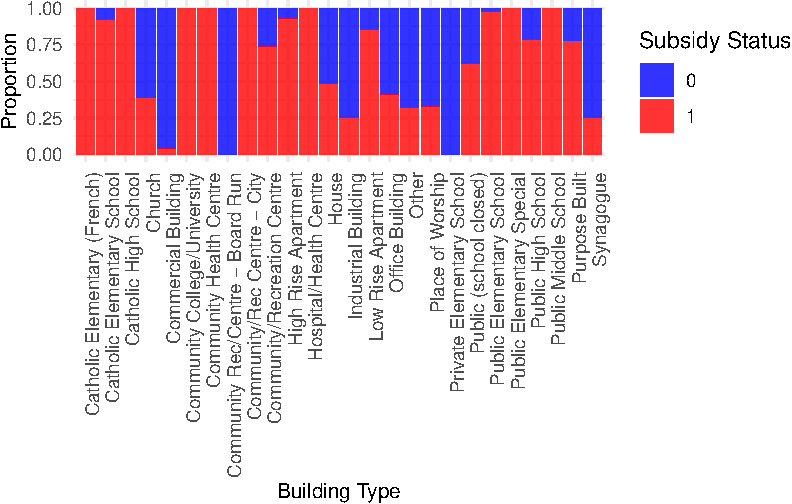
\includegraphics{paper_files/figure-pdf/fig-relationbldgtype-1.pdf}

}

\caption{\label{fig-relationbldgtype}Proportional Distribution of
Subsidy Status Across Building Types}

\end{figure}%

Figure~\ref{fig-relationAuspice} illustrates the proportional
distribution of subsidy status (1 = Subsidized, 0 = Not Subsidized)
across the different operating auspices of licensed child care centres:
Commercial Agency, Non-Profit Agency, and Other. Non-Profit Agencies and
``Other'' entities are predominantly subsidized, while Commercial
Agencies display a more balanced distribution. This aligns with research
indicating that non-profits rely heavily on subsidies to deliver public
goods and services, as they often operate in markets with limited
profitability (Hansmann 1979). Conversely, commercial entities are less
reliant on subsidies due to their revenue-driven models.The dominance of
subsidies in the ``Other'' category suggests this group may include
hybrid or public-private organizations aligned with specific government
initiatives (Anheier 2014). Such reliance reflects the strategic use of
subsidies to support services underserved by the private market
(Weisbrod 2000).

\begin{figure}

\centering{

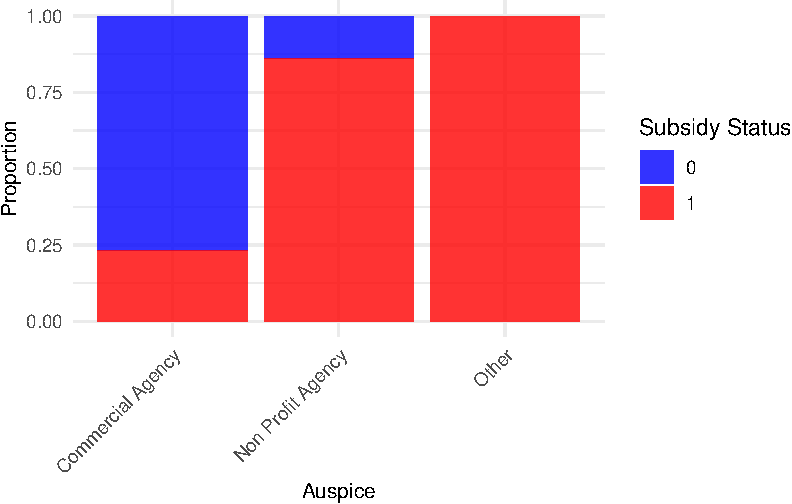
\includegraphics{paper_files/figure-pdf/fig-relationAuspice-1.pdf}

}

\caption{\label{fig-relationAuspice}Proportional Distribution of Subsidy
Status by Auspice}

\end{figure}%

Figure~\ref{fig-key} a heatmap illustrates the correlations between
three variables: TOTSPACE (likely representing total space or capacity),
subsidy (indicating subsidy status or amount), and cwelcc\_flag
(potentially denoting eligibility for a specific program or funding).
The positive correlation between TOTSPACE and subsidy (0.25) suggests
that larger facilities are modestly more likely to receive subsidies,
reflecting their capacity to serve larger populations or provide greater
public benefits. This aligns with research indicating that larger
organizations often have the resources and visibility to secure
subsidies (Hansmann, 1980; Salamon, 2002). Additionally, the stronger
correlation between subsidy and cwelcc\_flag (0.48) highlights that
subsidy allocation may target entities meeting specific programmatic or
policy criteria, consistent with the literature emphasizing strategic
targeting of subsidies to maximize societal impact (Weisbrod, 1998). The
weaker correlation between TOTSPACE and cwelcc\_flag (0.17) suggests
that program eligibility is less dependent on size and more on
qualitative factors like service type or demographic focus, which is
supported by Anheier's (2005) analysis of non-profit funding models.
Together, these correlations emphasize the nuanced role of subsidies in
balancing operational scale and policy alignment, underscoring the
importance of strategic allocation in public funding (Salamon, 1995).

\begin{figure}

\centering{

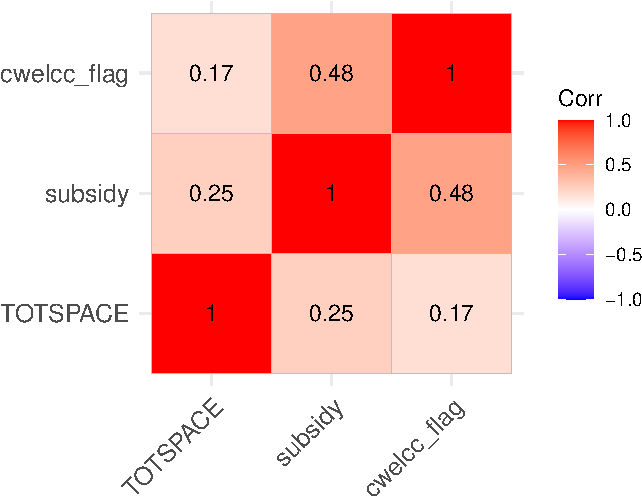
\includegraphics{paper_files/figure-pdf/fig-key-1.pdf}

}

\caption{\label{fig-key}Correlation Heatmap of Key Variables: TOTSPACE,
Subsidy, and CWELCC Flag}

\end{figure}%

\section{Model}\label{model}

\subsection{Model Specification}\label{model-specification}

To investigate the factors influencing subsidy allocation to licensed
child care centres, a reduced logistic regression model was specified.
The dependent variable,\texttt{subsidy}, is a binary indicator
representing whether a child care centre receives government subsidy (1
= subsidized, 0 = not subsidized). The model includes three key
predictors: \texttt{Operating\ Auspice\ (AUSPICE)}: A categorical
variable indicating the governance model of the child care centre (e.g.,
Non-Profit Agency, Other). Non-profit agencies are hypothesized to be
positively associated with subsidy allocation, consistent with previous
research emphasizing their prioritization in funding schemes (Cleveland
\& Krashinsky, 2005).
\texttt{Participation\ in\ the\ CWELCC\ Program\ (cwelcc\_flag)}: A
binary variable capturing whether the centre participates in the
Canada-Wide Early Learning and Child Care program (1 = participates, 0 =
does not participate). Centres participating in this initiative are
expected to have higher odds of receiving subsidies due to their
alignment with government objectives of affordability and accessibility
(Friendly \& Ballantyne, 2022). \texttt{Total\ Space\ (TOTSPACE)}: A
continuous variable representing the number of licensed spaces available
in the centre. Larger centres are hypothesized to have higher odds of
subsidy allocation, as they can accommodate more families and align with
policy goals of maximizing access (Forry et al., 2010). The logistic
regression model can be expressed mathematically as follows:

\subsection{Model Justification}\label{model-justification}

The logistic regression model was chosen for this analysis because it is
well-suited to the binary nature of the dependent variable, subsidy
status (1 = Subsidized, 0 = Not Subsidized). A logistic regression model
using the binomial family is specifically designed to model dichotomous
outcomes by estimating the log-odds of the event occurring as a linear
function of predictor variables (Hosmer Jr, Lemeshow, and Sturdivant
2013). The binomial family is appropriate here because it assumes that
the dependent variable follows a Bernoulli distribution, where each
observation represents a binary outcome (subsidized or not subsidized).
This ensures that the predicted probabilities remain between 0 and 1,
aligning with the real-world constraints of the problem. Additionally,
logistic regression provides interpretable coefficients, which indicate
the direction and magnitude of the relationship between each predictor
and the log-odds of subsidy allocation. This makes it particularly
useful for guiding policy decisions, as coefficients can be directly
converted into odds ratios for actionable insights (Peng, Lee, and
Ingersoll 2002). The ward variable was excluded because it lacked
statistical significance and added redundancy, as its effects were
captured by other predictors like CWELCC participation and total space.
Additionally, ward had no strong theoretical justification as a direct
determinant of subsidy allocation. The building type variable was
removed due to high dimensionality, sparse representation in many
categories, and statistical insignificance. Its effects are likely
mediated by other variables, such as total space and auspice. Excluding
it improved parsimony and interpretability. The final model retained
operating auspice, CWELCC participation, and total space, as these
predictors are strongly supported by theory and data. This approach
balances simplicity and accuracy, ensuring the model remains relevant
for informing equitable subsidy allocation policies.

\subsection{Model Assumptions}\label{model-assumptions}

To ensure the validity of the logistic regression model, several key
assumptions were assessed, including independence of observations, the
appropriateness of a binary outcome, the linearity of predictors with
the logit and absence of multicollinearity. The analysis integrates
results from visual diagnostics, multicollinearity tests, and
statistical measures. 1. Independence of Observations The logistic
regression model assumes that the observations are independent of each
other. In this analysis, each data point corresponds to an individual
child care center, ensuring independence. There is no clustering or
repeated measures within the dataset, which validates this assumption.
2. Binary Outcome The logistic regression model assumes a binary
dependent variable. In this case, the outcome variable,
\texttt{subsidy}, is binary, indicating whether a child care center
receives a subsidy (1 = Subsidized, 0 = Not Subsidized). This aligns
with the model's requirement, ensuring the suitability of the binomial
family for fitting the data. 3. Linearity of Predictors with the Logit
The Figure~\ref{fig-cr} The component + residual plots evaluate the
linearity of the continuous variables and the relationship between
categorical predictors and the logit transformation. graph

\begin{figure}

\centering{

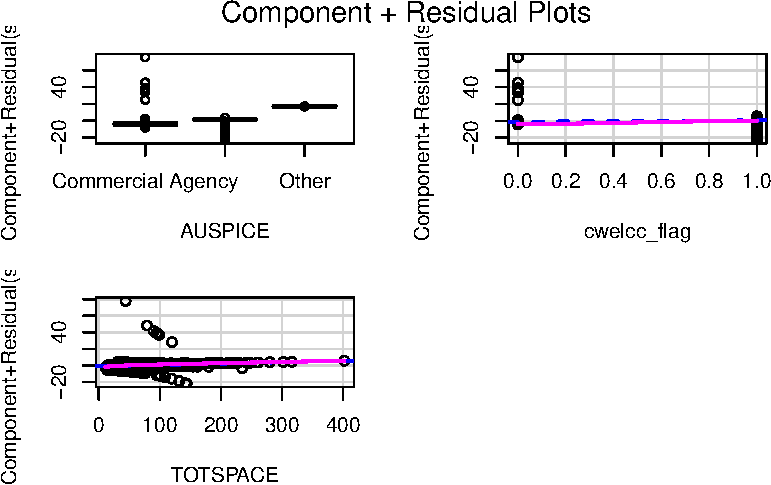
\includegraphics{paper_files/figure-pdf/fig-cr-1.pdf}

}

\caption{\label{fig-cr}CR Plot for Linearity Chekck}

\end{figure}%

\texttt{TOTSPACE}: The relationship between the total space (TOTSPACE)
and the logit appears approximately linear, as indicated by the flat,
consistent pattern of residuals around the horizontal axis. This
supports the assumption of linearity. \texttt{CWELCC\ Flag}: The plot
for CWELCC participation shows a horizontal trend, suggesting no
significant deviation from linearity. The data support the inclusion of
this variable as a binary predictor. \texttt{AUSPICE}: The residual
patterns for categorical levels of AUSPICE (e.g., ``Commercial Agency''
and ``Other'') indicate distinct clusters with consistent variability.
This suggests the categorical nature of this variable does not violate
linearity assumptions. Overall, the visual inspection suggests that the
linearity assumption for the predictors with the logit is met.

\begin{enumerate}
\def\labelenumi{\arabic{enumi}.}
\setcounter{enumi}{3}
\tightlist
\item
  Multicollinearity Assessment Variance Inflation Factor (VIF): To
  assess multicollinearity among the predictors, the VIF values for the
  reduced model variables were calculated.
\end{enumerate}

\begin{Shaded}
\begin{Highlighting}[]
\CommentTok{\# Calculate VIF}
\NormalTok{vif\_values }\OtherTok{\textless{}{-}} \FunctionTok{vif}\NormalTok{(reduced\_model\_2)}
\end{Highlighting}
\end{Shaded}

All VIF values are below 2, well within the acceptable threshold of 5,
indicating minimal multicollinearity among the predictors. The
independence of the predictors ensures the stability of the coefficient
estimates.

\subsection{Alternative Models}\label{alternative-models}

Alternative models like decision trees and random forests were
considered but were found less interpretable for policy-focused
analyses. Logistic regression was chosen for its balance of simplicity,
interpretability, and effectiveness.

\#Result The logistic regression model's performance metrics are
presented in Table~\ref{tbl-coefresult}.

\begin{table}

\caption{\label{tbl-coefresult}Regression Result}

\centering{

\centering
\begin{tblr}[         %% tabularray outer open
]                     %% tabularray outer close
{                     %% tabularray inner open
colspec={Q[]Q[]},
column{1}={halign=l,},
column{2}={halign=c,},
hline{17}={1,2}{solid, 0.05em, black},
}                     %% tabularray inner close
\toprule
& Final Model \\ \midrule %% TinyTableHeader
(Intercept)              & -4.967    \\
& (0.496)   \\
& (<0.001)  \\
AUSPICENon Profit Agency & 2.883     \\
& (0.234)   \\
& (<0.001)  \\
AUSPICEOther             & 18.772    \\
& (686.847) \\
& (0.978)   \\
cwelcc_flag              & 3.156     \\
& (0.436)   \\
& (<0.001)  \\
TOTSPACE                 & 0.014     \\
& (0.003)   \\
& (<0.001)  \\
Num.Obs.                 & 750       \\
AIC                      & 528.1     \\
BIC                      & 551.2     \\
Log.Lik.                 & -259.035  \\
RMSE                     & 0.32      \\
\bottomrule
\end{tblr}

}

\end{table}%

The regression model reveals several key observations regarding the
predictors and overall goodness of fit. The intercept, estimated at
-4.967, represents the baseline log-odds of the outcome when all
predictors are at their reference or zero level. While not directly
interpretable, it serves as a baseline reference for the model. Among
the predictors, the AUSPICE: Non-Profit Agency category significantly
increases the log-odds of the outcome, with an estimate of 2.883 and a
small standard error of 0.234, indicating a strong and reliable positive
effect. However, the AUSPICE: Other category shows an unusually large
coefficient (18.772) paired with a very high standard error (686.847),
suggesting instability. The CWELCC Flag variable also exhibits a strong
and reliable positive effect, with an estimate of 3.156 and a standard
error of 0.436, indicating that being flagged as CWELCC significantly
increases the log-odds of the outcome. Additionally, the TOTSPACE
variable has a small but statistically significant effect, with an
estimate of 0.014 and a low standard error of 0.003, reflecting
robustness.

In terms of model fit, the dataset includes 750 observations, and the
model's AIC (528.1) and BIC (551.2) suggest a reasonable balance between
goodness of fit and complexity, as lower values are generally preferred
(Burnham and Anderson, n.d.). The log-likelihood of -259.035 also
supports an adequate fit, with a higher (less negative) value indicating
better alignment between the model and the data. Finally, the RMSE of
0.32 reflects the model's predictive accuracy, with a low value
indicating that the model's predictions closely match the observed data.
Overall, the model performs well but may require refinement,
particularly in addressing instability in the AUSPICE: Other variable.

The evaluation of the logistic regression model shows strong performance
based on McFadden's R\^{}2 and the Area Under the Receiver Operating
Characteristic Curve (AUC). McFadden's R\^{}2 which is a pseudo-R\^{}2
metric specifically designed for logistic regression, was calculated as
0.454. This value suggests that the model explains 45.4\% of the
variance in the outcome variable, indicating a well-fitting model.
McFadden (\textbf{mcfadden1972conditional?}) proposed this metric as a
reliable measure for logistic regression, where values between 0.2 and
0.4 are considered indicative of a good model fit, and values above 0.4
demonstrate an excellent fit. Thus, the model's R\^{}2 value strongly
supports its utility in predicting the outcome.

\begin{Shaded}
\begin{Highlighting}[]
\CommentTok{\# Extract coefficients and confidence intervals}
\NormalTok{tidy\_model }\OtherTok{\textless{}{-}}\NormalTok{ broom}\SpecialCharTok{::}\FunctionTok{tidy}\NormalTok{(reduced\_model\_2, }\AttributeTok{conf.int =} \ConstantTok{TRUE}\NormalTok{)}
\end{Highlighting}
\end{Shaded}

\begin{verbatim}
Warning: glm.fit: fitted probabilities numerically 0 or 1 occurred
Warning: glm.fit: fitted probabilities numerically 0 or 1 occurred
Warning: glm.fit: fitted probabilities numerically 0 or 1 occurred
Warning: glm.fit: fitted probabilities numerically 0 or 1 occurred
Warning: glm.fit: fitted probabilities numerically 0 or 1 occurred
Warning: glm.fit: fitted probabilities numerically 0 or 1 occurred
Warning: glm.fit: fitted probabilities numerically 0 or 1 occurred
Warning: glm.fit: fitted probabilities numerically 0 or 1 occurred
Warning: glm.fit: fitted probabilities numerically 0 or 1 occurred
Warning: glm.fit: fitted probabilities numerically 0 or 1 occurred
Warning: glm.fit: fitted probabilities numerically 0 or 1 occurred
Warning: glm.fit: fitted probabilities numerically 0 or 1 occurred
Warning: glm.fit: fitted probabilities numerically 0 or 1 occurred
Warning: glm.fit: fitted probabilities numerically 0 or 1 occurred
Warning: glm.fit: fitted probabilities numerically 0 or 1 occurred
Warning: glm.fit: fitted probabilities numerically 0 or 1 occurred
Warning: glm.fit: fitted probabilities numerically 0 or 1 occurred
Warning: glm.fit: fitted probabilities numerically 0 or 1 occurred
Warning: glm.fit: fitted probabilities numerically 0 or 1 occurred
Warning: glm.fit: fitted probabilities numerically 0 or 1 occurred
Warning: glm.fit: fitted probabilities numerically 0 or 1 occurred
Warning: glm.fit: fitted probabilities numerically 0 or 1 occurred
\end{verbatim}

\begin{Shaded}
\begin{Highlighting}[]
\CommentTok{\# Highlight significant coefficients}
\NormalTok{tidy\_model }\OtherTok{\textless{}{-}}\NormalTok{ tidy\_model }\SpecialCharTok{\%\textgreater{}\%}
  \FunctionTok{mutate}\NormalTok{(}\AttributeTok{significant =} \FunctionTok{ifelse}\NormalTok{(conf.low }\SpecialCharTok{\textgreater{}} \DecValTok{0} \SpecialCharTok{|}\NormalTok{ conf.high }\SpecialCharTok{\textless{}} \DecValTok{0}\NormalTok{, }\StringTok{"Significant"}\NormalTok{, }\StringTok{"Not Significant"}\NormalTok{))}

\CommentTok{\# Plot with enhancements}
\FunctionTok{ggplot}\NormalTok{(tidy\_model, }\FunctionTok{aes}\NormalTok{(}\AttributeTok{x =}\NormalTok{ estimate, }\AttributeTok{y =} \FunctionTok{reorder}\NormalTok{(term, }\FunctionTok{abs}\NormalTok{(estimate)), }\AttributeTok{color =}\NormalTok{ significant)) }\SpecialCharTok{+}
  \FunctionTok{geom\_point}\NormalTok{() }\SpecialCharTok{+}
  \FunctionTok{geom\_errorbarh}\NormalTok{(}\FunctionTok{aes}\NormalTok{(}\AttributeTok{xmin =}\NormalTok{ conf.low, }\AttributeTok{xmax =}\NormalTok{ conf.high), }\AttributeTok{height =} \FloatTok{0.2}\NormalTok{) }\SpecialCharTok{+}
  \FunctionTok{scale\_color\_manual}\NormalTok{(}\AttributeTok{values =} \FunctionTok{c}\NormalTok{(}\StringTok{"Significant"} \OtherTok{=} \StringTok{"red"}\NormalTok{, }\StringTok{"Not Significant"} \OtherTok{=} \StringTok{"black"}\NormalTok{)) }\SpecialCharTok{+}
  \FunctionTok{labs}\NormalTok{(}
    \AttributeTok{title =} \StringTok{"Coefficient Plot"}\NormalTok{,}
    \AttributeTok{x =} \StringTok{"Coefficient Estimate"}\NormalTok{,}
    \AttributeTok{y =} \StringTok{"Predictor Variables"}\NormalTok{,}
    \AttributeTok{color =} \StringTok{"Significance"}
\NormalTok{  ) }\SpecialCharTok{+}
  \FunctionTok{theme\_minimal}\NormalTok{()}
\end{Highlighting}
\end{Shaded}

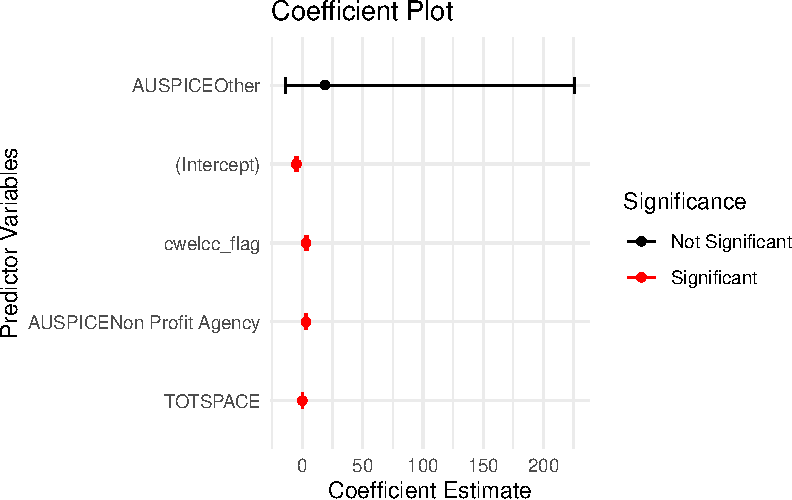
\includegraphics{paper_files/figure-pdf/unnamed-chunk-16-1.pdf}

\begin{Shaded}
\begin{Highlighting}[]
\CommentTok{\# Calculate log{-}likelihood of the fitted model}
\NormalTok{log\_likelihood\_fitted }\OtherTok{\textless{}{-}} \FunctionTok{logLik}\NormalTok{(reduced\_model\_2)}
\CommentTok{\# Fit the null model (model with intercept only)}
\NormalTok{null\_model }\OtherTok{\textless{}{-}} \FunctionTok{glm}\NormalTok{(subsidy }\SpecialCharTok{\textasciitilde{}} \DecValTok{1}\NormalTok{, }\AttributeTok{data =}\NormalTok{ train\_data, }\AttributeTok{family =}\NormalTok{ binomial)}
\NormalTok{log\_likelihood\_null }\OtherTok{\textless{}{-}} \FunctionTok{logLik}\NormalTok{(null\_model)}
\CommentTok{\# McFadden\textquotesingle{}s R{-}squared}
\NormalTok{mcfadden\_r2 }\OtherTok{\textless{}{-}} \DecValTok{1} \SpecialCharTok{{-}} \FunctionTok{as.numeric}\NormalTok{(log\_likelihood\_fitted }\SpecialCharTok{/}\NormalTok{ log\_likelihood\_null)}
\CommentTok{\# Print the result}
\FunctionTok{print}\NormalTok{(}\FunctionTok{paste}\NormalTok{(}\StringTok{"McFadden\textquotesingle{}s R{-}squared:"}\NormalTok{, }\FunctionTok{round}\NormalTok{(mcfadden\_r2, }\DecValTok{6}\NormalTok{)))}
\end{Highlighting}
\end{Shaded}

\begin{verbatim}
[1] "McFadden's R-squared: 0.454164"
\end{verbatim}

\begin{verbatim}
Area under the curve: 0.8998
\end{verbatim}

\begin{figure}

\centering{

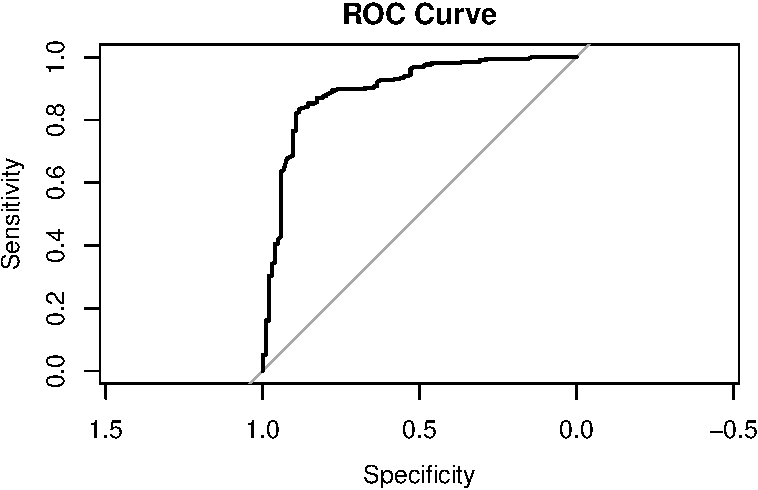
\includegraphics{paper_files/figure-pdf/fig-roc-1.pdf}

}

\caption{\label{fig-roc}ROC Curve for Model Performance}

\end{figure}%

The ROC curve in Figure~\ref{fig-roc} shown further validates the
model's classification ability, with an AUC of 0.8998. An AUC value
close to 1 indicates excellent discriminative power, where the model
effectively separates true positives from false positives. The AUC of
0.8998 places this model on the borderline of very good and excellent
discrimination, underscoring its robust predictive capacity. These
results collectively suggest that the logistic regression model not only
fits the data well but also performs strongly in classification tasks.
However, as suggested by Harrell (Harrell 2012), care must be taken to
ensure the model is not overfitted, particularly given the high AUC
value. Cross-validation or testing on an independent dataset is
recommended to confirm the model's generalizability. Additionally,
assessing the contribution of individual predictors can enhance the
interpretability of the model, as overly complex models may inflate
performance metrics without offering meaningful insights. Overall, the
model's performance metrics strongly support its use for prediction in
practical settings while aligning with academic standards for model
evaluation.

\begin{Shaded}
\begin{Highlighting}[]
\CommentTok{\# Generate predicted probabilities for the test dataset}
\NormalTok{test\_data}\SpecialCharTok{$}\NormalTok{predicted\_prob }\OtherTok{\textless{}{-}} \FunctionTok{predict}\NormalTok{(reduced\_model\_2, }\AttributeTok{newdata =}\NormalTok{ test\_data, }\AttributeTok{type =} \StringTok{"response"}\NormalTok{)}

\CommentTok{\# Predicted vs. Observed Scatterplot}
\FunctionTok{ggplot}\NormalTok{(test\_data, }\FunctionTok{aes}\NormalTok{(}\AttributeTok{x =}\NormalTok{ predicted\_prob, }\AttributeTok{y =}\NormalTok{ subsidy)) }\SpecialCharTok{+}
  \FunctionTok{geom\_jitter}\NormalTok{(}\AttributeTok{width =} \FloatTok{0.02}\NormalTok{, }\AttributeTok{height =} \FloatTok{0.02}\NormalTok{, }\AttributeTok{alpha =} \FloatTok{0.6}\NormalTok{, }\AttributeTok{color =} \StringTok{"blue"}\NormalTok{) }\SpecialCharTok{+}
  \FunctionTok{geom\_smooth}\NormalTok{(}\AttributeTok{method =} \StringTok{"loess"}\NormalTok{, }\AttributeTok{color =} \StringTok{"red"}\NormalTok{, }\AttributeTok{se =} \ConstantTok{FALSE}\NormalTok{) }\SpecialCharTok{+}
  \FunctionTok{labs}\NormalTok{(}
    \AttributeTok{title =} \StringTok{"Predicted vs. Observed Probability"}\NormalTok{,}
    \AttributeTok{x =} \StringTok{"Predicted Probability"}\NormalTok{,}
    \AttributeTok{y =} \StringTok{"Observed Outcome"}
\NormalTok{  ) }\SpecialCharTok{+}
  \FunctionTok{theme\_minimal}\NormalTok{()}
\end{Highlighting}
\end{Shaded}

\begin{verbatim}
`geom_smooth()` using formula = 'y ~ x'
\end{verbatim}

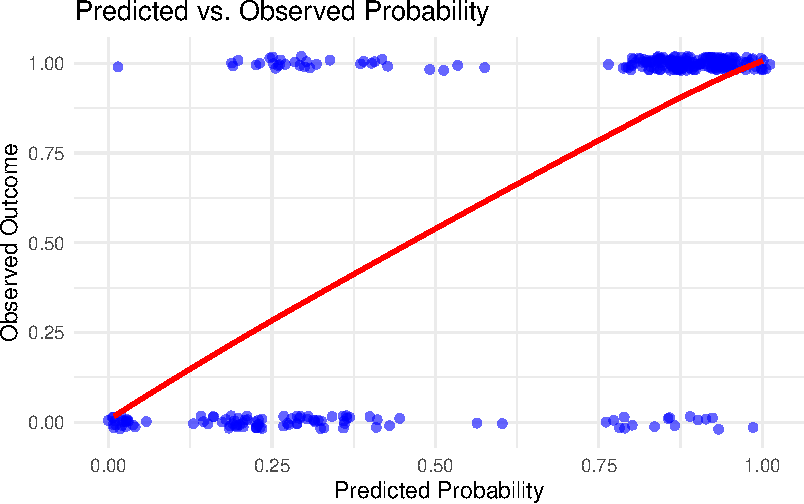
\includegraphics{paper_files/figure-pdf/unnamed-chunk-19-1.pdf}

\begin{Shaded}
\begin{Highlighting}[]
\CommentTok{\# Create a coefficient table}
\NormalTok{model\_list }\OtherTok{\textless{}{-}} \FunctionTok{list}\NormalTok{(}
  \StringTok{"Full Model"} \OtherTok{=}\NormalTok{ log\_model,}
  \StringTok{"AIC Model"} \OtherTok{=}\NormalTok{ reduced\_model\_re,}
  \StringTok{"Simplified Model"} \OtherTok{=}\NormalTok{ reduced\_model\_2}
\NormalTok{)}

\CommentTok{\# Customize the table to display only AIC and Deviance}
\FunctionTok{modelsummary}\NormalTok{(}
\NormalTok{  model\_list,}
  \AttributeTok{output =} \StringTok{"markdown"}\NormalTok{,}
  \AttributeTok{gof\_map =} \FunctionTok{c}\NormalTok{(}\StringTok{"AIC"}\NormalTok{, }\StringTok{"Deviance"}\NormalTok{)  }\CommentTok{\# Include only AIC and Deviance in the table}
\NormalTok{)}
\end{Highlighting}
\end{Shaded}

\begin{table}
\centering
\begin{tblr}[         %% tabularray outer open
]                     %% tabularray outer close
{                     %% tabularray inner open
colspec={Q[]Q[]Q[]Q[]},
column{1}={halign=l,},
column{2}={halign=c,},
column{3}={halign=c,},
column{4}={halign=c,},
}                     %% tabularray inner close
\toprule
& Full Model & AIC Model & Simplified Model \\ \midrule %% TinyTableHeader
(Intercept)                               & 10.717     & 10.655     & -4.967    \\
& (2454.170) & (2457.796) & (0.496)   \\
ward                                      & -0.007     &            &           \\
& (0.021)    &            &           \\
AUSPICENon Profit Agency                  & 2.752      & 2.753      & 2.883     \\
& (0.339)    & (0.339)    & (0.234)   \\
AUSPICEOther                              & 19.252     & 19.261     & 18.772    \\
& (1009.264) & (1008.865) & (686.847) \\
bldg_typeCatholic Elementary School       & -14.928    & -14.930    &           \\
& (2454.170) & (2457.796) &           \\
bldg_typeCatholic High School             & 1.120      & 1.037      &           \\
& (6969.058) & (6970.335) &           \\
bldg_typeChurch                           & -16.826    & -16.826    &           \\
& (2454.170) & (2457.796) &           \\
bldg_typeCommercial Building              & -18.590    & -18.616    &           \\
& (2454.171) & (2457.796) &           \\
bldg_typeCommunity College/University     & 1.009      & 0.989      &           \\
& (4488.740) & (4490.254) &           \\
bldg_typeCommunity Health Centre          & 1.092      & 1.037      &           \\
& (6969.058) & (6970.335) &           \\
bldg_typeCommunity Rec/Centre - Board Run & -35.148    & -35.072    &           \\
& (6969.058) & (6970.335) &           \\
bldg_typeCommunity/Rec Centre - City      & 1.053      & 1.077      &           \\
& (4061.162) & (4063.980) &           \\
bldg_typeCommunity/Recreation Centre      & -16.003    & -16.013    &           \\
& (2454.170) & (2457.796) &           \\
bldg_typeHigh Rise Apartment              & -12.625    & -12.631    &           \\
& (2454.170) & (2457.796) &           \\
bldg_typeHospital/Health Centre           & 1.367      & 1.354      &           \\
& (6969.058) & (6970.335) &           \\
bldg_typeHouse                            & -14.939    & -14.920    &           \\
& (2454.170) & (2457.796) &           \\
bldg_typeIndustrial Building              & -32.542    & -32.470    &           \\
& (4618.831) & (4622.295) &           \\
bldg_typeLow Rise Apartment               & -14.884    & -14.852    &           \\
& (2454.173) & (2457.798) &           \\
bldg_typeOffice Building                  & -16.708    & -16.695    &           \\
& (2454.170) & (2457.796) &           \\
bldg_typeOther                            & -16.973    & -16.963    &           \\
& (2454.170) & (2457.796) &           \\
bldg_typePlace of Worship                 & -16.929    & -16.931    &           \\
& (2454.170) & (2457.796) &           \\
bldg_typePrivate Elementary School        & -34.849    & -34.836    &           \\
& (3381.477) & (3387.732) &           \\
bldg_typePublic (school closed)           & -16.221    & -16.188    &           \\
& (2454.170) & (2457.796) &           \\
bldg_typePublic Elementary School         & -13.716    & -13.712    &           \\
& (2454.170) & (2457.796) &           \\
bldg_typePublic Elementary Special        & -0.010     & 0.007      &           \\
& (6969.058) & (6970.335) &           \\
bldg_typePublic High School               & -15.904    & -15.871    &           \\
& (2454.170) & (2457.796) &           \\
bldg_typePublic Middle School             & 1.045      & 1.117      &           \\
& (6969.058) & (6970.335) &           \\
bldg_typePurpose Built                    & -14.567    & -14.572    &           \\
& (2454.170) & (2457.796) &           \\
bldg_typeSynagogue                        & -18.451    & -18.405    &           \\
& (2454.170) & (2457.796) &           \\
cwelcc_flag                               & 3.504      & 3.473      & 3.156     \\
& (0.519)    & (0.510)    & (0.436)   \\
TOTSPACE                                  & 0.013      & 0.013      & 0.014     \\
& (0.004)    & (0.004)    & (0.003)   \\
\bottomrule
\end{tblr}
\end{table}

\section*{References}\label{references}
\addcontentsline{toc}{section}{References}

\phantomsection\label{refs}
\begin{CSLReferences}{1}{0}
\bibitem[\citeproctext]{ref-anheier2014nonprofit}
Anheier, Helmut K. 2014. \emph{Nonprofit Organizations: Theory,
Management, Policy}. Routledge.

\bibitem[\citeproctext]{ref-burnhammodel}
Burnham, KP, and DR Anderson. n.d. {``Model Selection and Multimodel
Inference: A Practical Information-Theoretic Approach2nd Ed.
2002Springer-Verlag.''} \emph{New York}.

\bibitem[\citeproctext]{ref-cleveland2009nonprofit}
Cleveland, Gordon, and Michael Krashinsky. 2009. {``The Nonprofit
Advantage: Producing Quality in Thick and Thin Child Care Markets.''}
\emph{Journal of Policy Analysis and Management} 28 (3): 440--62.

\bibitem[\citeproctext]{ref-citecar}
Fox, John, and Sanford Weisberg. 2019. \emph{An {R} Companion to Applied
Regression}. Third. Thousand Oaks {CA}: Sage.
\url{https://www.john-fox.ca/Companion/}.

\bibitem[\citeproctext]{ref-citeopendatatoronto}
Gelfand, Sharla. 2022. \emph{Opendatatoronto: Access the City of Toronto
Open Data Portal}.
\url{https://CRAN.R-project.org/package=opendatatoronto}.

\bibitem[\citeproctext]{ref-hansmann1979role}
Hansmann, Henry B. 1979. {``The Role of Nonprofit Enterprise.''}
\emph{Yale LJ} 89: 835.

\bibitem[\citeproctext]{ref-harrell2012regression}
Harrell, Frank E. 2012. {``Regression Modeling Strategies.''} \emph{R
Package Version}, 6--2.

\bibitem[\citeproctext]{ref-citestagazer}
Hlavac, Marek. 2022. \emph{Stargazer: Well-Formatted Regression and
Summary Statistics Tables}. Bratislava, Slovakia: Social Policy
Institute. \url{https://CRAN.R-project.org/package=stargazer}.

\bibitem[\citeproctext]{ref-hosmer2013applied}
Hosmer Jr, David W, Stanley Lemeshow, and Rodney X Sturdivant. 2013.
\emph{Applied Logistic Regression}. John Wiley \& Sons.

\bibitem[\citeproctext]{ref-Johnson_Ryan_Brooks_2012}
Johnson, Anna D., Rebecca M. Ryan, and Jeanne Brooks‐Gunn. 2012.
{``Child‐care Subsidies: Do They Impact the Quality of Care Children
Experience?''} \emph{Child Development} 83 (4): 1444--61.
\url{https://doi.org/10.1111/j.1467-8624.2012.1780.x}.

\bibitem[\citeproctext]{ref-citecaret}
Kuhn, and Max. 2008. {``Building Predictive Models in r Using the Caret
Package.''} \emph{Journal of Statistical Software} 28 (5): 1--26.
\url{https://doi.org/10.18637/jss.v028.i05}.

\bibitem[\citeproctext]{ref-peng2002introduction}
Peng, Chao-Ying Joanne, Kuk Lida Lee, and Gary M Ingersoll. 2002. {``An
Introduction to Logistic Regression Analysis and Reporting.''} \emph{The
Journal of Educational Research} 96 (1): 3--14.

\bibitem[\citeproctext]{ref-citeR}
R Core Team. 2023. \emph{{R: A Language and Environment for Statistical
Computing}}. Vienna, Austria: R Foundation for Statistical Computing.
\url{https://www.R-project.org/}.

\bibitem[\citeproctext]{ref-ryan2011impact}
Ryan, Rebecca M, Anna Johnson, Elizabeth Rigby, and Jeanne Brooks-Gunn.
2011. {``The Impact of Child Care Subsidy Use on Child Care Quality.''}
\emph{Early Childhood Research Quarterly} 26 (3): 320--31.

\bibitem[\citeproctext]{ref-vines2020accessing}
Vines, Shere'lle Ramsey. 2020. {``Accessing Equity: Challenges
Middle-Income Families Face Finding High Quality Childcare.''}

\bibitem[\citeproctext]{ref-weisbrod2000profit}
Weisbrod, Burton A. 2000. \emph{To Profit or Not to Profit: The
Commercial Transformation of the Nonprofit Sector}. Cambridge University
Press.

\bibitem[\citeproctext]{ref-citeggplot2}
Wickham, Hadley. 2016. \emph{Ggplot2: Elegant Graphics for Data
Analysis}. Springer-Verlag New York.
\url{https://ggplot2.tidyverse.org}.

\bibitem[\citeproctext]{ref-citetidyverse}
Wickham, Hadley, Mara Averick, Jennifer Bryan, Winston Chang, Lucy
D'Agostino McGowan, Romain François, Garrett Grolemund, et al. 2019.
{``Welcome to the {tidyverse}.''} \emph{Journal of Open Source Software}
4 (43): 1686. \url{https://doi.org/10.21105/joss.01686}.

\bibitem[\citeproctext]{ref-citedplyr}
Wickham, Hadley, Romain François, Lionel Henry, Kirill Müller, and Davis
Vaughan. 2023. \emph{Dplyr: A Grammar of Data Manipulation}.
\url{https://CRAN.R-project.org/package=dplyr}.

\bibitem[\citeproctext]{ref-citereadr}
Wickham, Hadley, Jim Hester, and Jennifer Bryan. 2024. \emph{Readr: Read
Rectangular Text Data}. \url{https://CRAN.R-project.org/package=readr}.

\bibitem[\citeproctext]{ref-citeknitr}
Xie, Yihui. 2021. \emph{Knitr: A General-Purpose Package for Dynamic
Report Generation in r}. \url{https://yihui.org/knitr/}.

\end{CSLReferences}




\end{document}
